% !TeX root = ../main.tex
\chapter{Unidad 1: Nociones básicas e introducción a la acústica}

\section{Objetivo pedagógico}
\noindent\textbf{Objetivo.} Introducir los conceptos fundamentales de la acústica, el Sistema Internacional de Unidades y las herramientas matemáticas básicas que utilizarás a lo largo de la asignatura. Estos conocimientos te permitirán entender cómo el sonido afecta la audición y la voz, y cómo se aplican en pruebas diagnósticas como audiometrías o en el diseño de audífonos. Se incluyen ejemplos, curiosidades clínicas y ejercicios pensados para estudiantes con escasa formación previa en matemáticas.

\noindent\textbf{Pregunta inicial.} ¿Alguna vez te preguntaste por qué un susurro suena diferente a un grito, o cómo un audífono mejora la audición? ¡Esta unidad te dará las bases para responder estas preguntas!

\section{¿Qué es la acústica?}
La \textbf{acústica} es la rama de la física que estudia las ondas mecánicas en gases, líquidos y sólidos. Estas ondas son vibraciones que viajan a través de un medio, como las ondas que se forman al tirar una piedra en un estanque. La acústica analiza cómo se \emph{genera} el sonido (por ejemplo, al hablar), cómo se \emph{propaga} (viaja por el aire), cómo \emph{interactúa} con el entorno (como un eco en una iglesia) y cómo lo \emph{percibe} el oído humano.

\subsection{Importancia en Fonoaudiología}
\begin{itemize}
    \item \textbf{Diagnóstico:} Las audiometrías, otoemisiones acústicas y potenciales evocados dependen de entender cómo viaja el sonido y cómo lo recibe el oído.
    \item \textbf{Rehabilitación:} El diseño de audífonos e implantes cocleares se basa en modelar la respuesta del sonido en el oído.
    \item \textbf{Análisis de la voz:} La acústica permite estudiar trastornos del habla, como la disfonía, analizando las frecuencias de la voz.
    \item \textbf{Ambientes clínicos:} Controlar el ruido de fondo en cabinas audiométricas es clave para obtener resultados precisos.
\end{itemize}

\begin{quote}
    \textbf{Dato curioso.} El término \textbf{acústica} proviene del griego \emph{akoustikos}, que significa ``relativo a la audición''. ¡Los antiguos griegos ya estudiaban cómo percibimos el sonido!
\end{quote}

\begin{figure}[h]
    \centering
    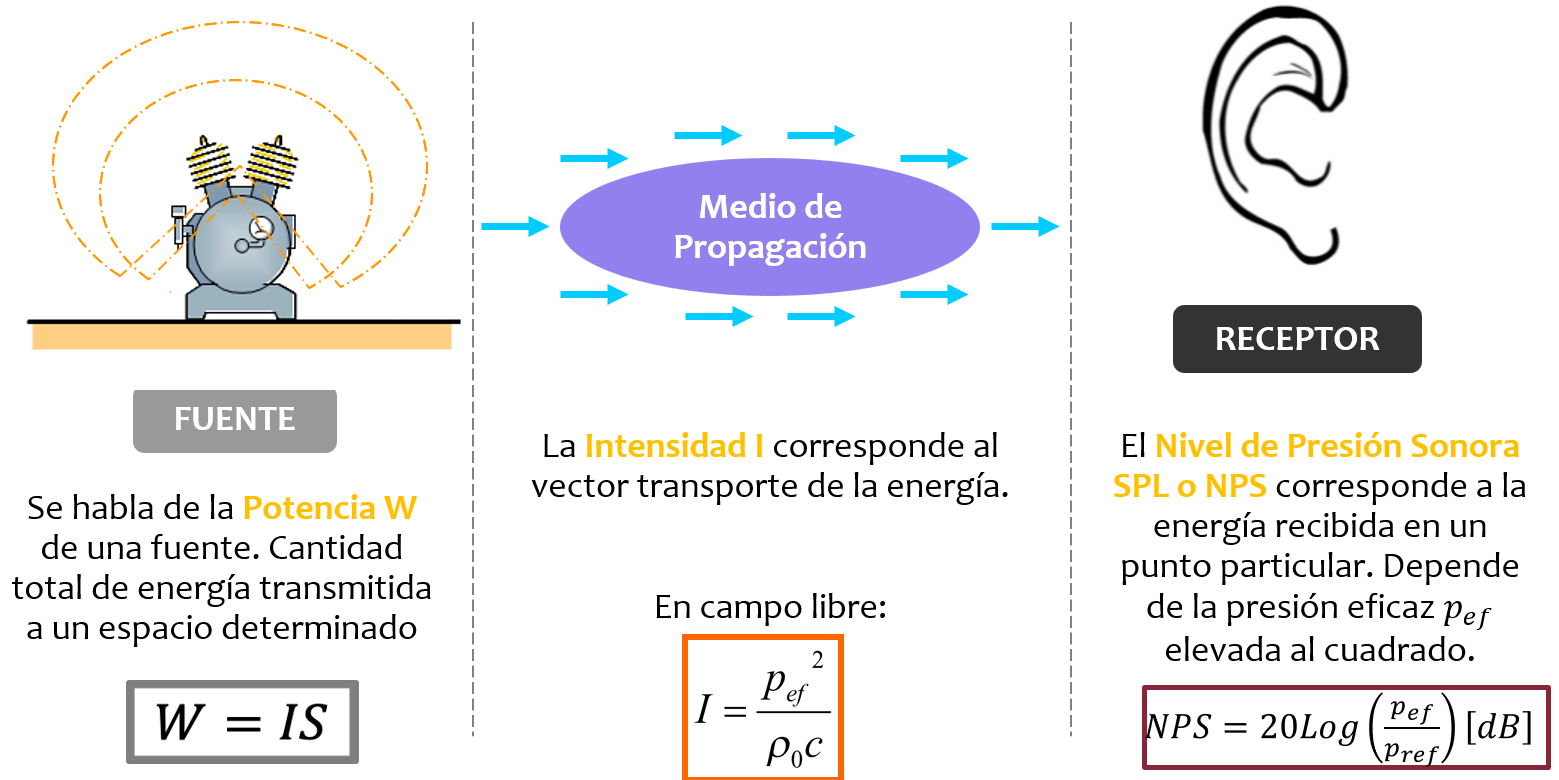
\includegraphics[width=1.0\textwidth]{figures/propagacion_sonido.png}
    \caption{ Diagrama simple de una onda sonora viajando desde una fuente hasta el oído humano a través de un medio de propagación.}
    \label{propagacion_sonido}
\end{figure}

\textbf{Recurso recomendado.} Video: \href{https://www.youtube.com/watch?v=qV4lR9EWGlY&ab_channel=CrashCourse}{``What is Sound?'' (Crash Course Physics).}  

\section{El sonido como onda mecánica}
Una onda sonora es una \emph{perturbación} que se propaga gracias a la elasticidad e inercia del medio, como el aire, el agua o el hueso. Imagina que golpeas un resorte: las compresiones viajan a lo largo de él, creando una onda. Así funciona el sonido en el aire, llevando la voz o la música hasta tu oído.

Es importante destacar que el sonido se propaga mediante ondas generadas por el movimiento oscilatorio de las partículas del medio, las cuales, tras transmitir la energía, regresan a su posición inicial. Este concepto es fundamental para comprender la transmisión del sonido en diferentes medios y será explorado en mayor detalle en capítulos posteriores.


\subsection{Tipos de ondas}
\begin{description}
    \item[\textbf{Ondas longitudinales:}] Las partículas del medio vibran en la misma dirección en que viaja la onda, creando zonas de compresión y rarefacción. Ejemplo: el sonido de tu voz viajando por el aire hasta el tímpano.
    \item[\textbf{Ondas transversales:}] Las partículas vibran perpendicularmente a la dirección de la onda. En fonoaudiología, estas ondas son relevantes en la audición ósea, cuando el cráneo vibra. Ejemplo: una cuerda de guitarra que vibra hacia arriba y abajo.
\end{description}

\begin{figure}[h]
    \centering
    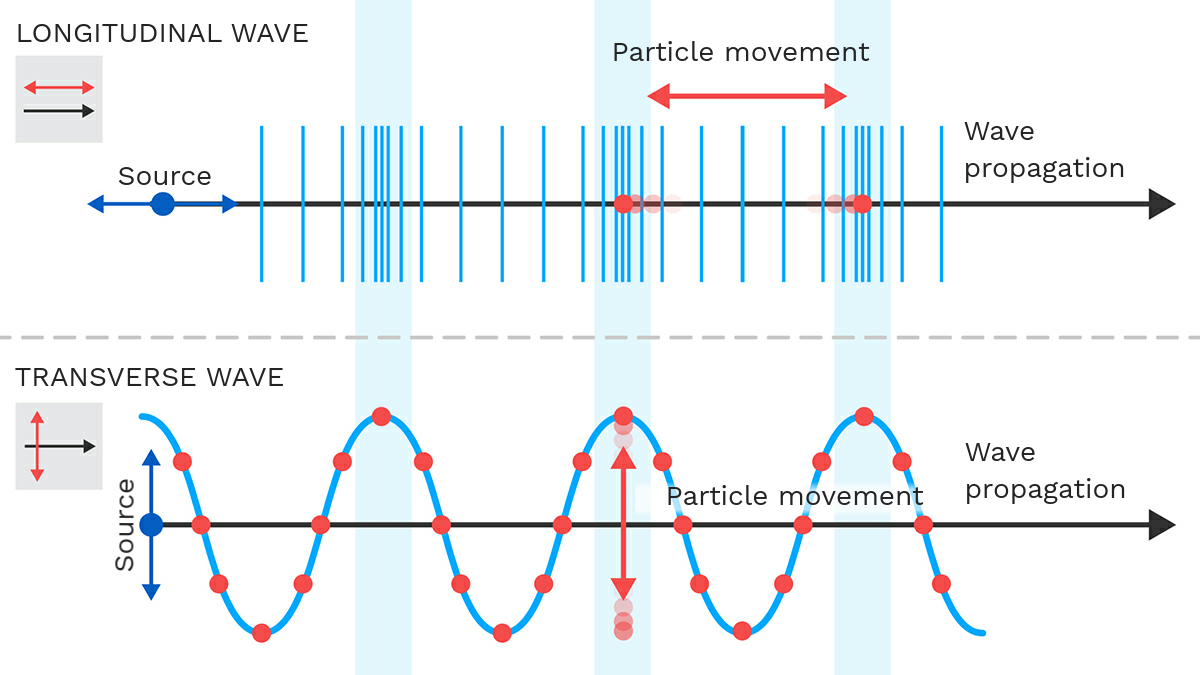
\includegraphics[width=1.0\textwidth]{figures/longitudinales_transversales.png}
    \caption{Comparativa de ondas longitudinales y transversales.}
    \label{fig:longitudinales-transversales}
\end{figure}

\textbf{Actividad práctica.} Usa un diapasón (o un video de un diapasón en YouTube) y un recipiente con agua. Golpea el diapasón para que vibre y acércalo al agua sin tocarla; escucha el sonido en el aire. Luego, sumerge parcialmente el diapasón en el agua mientras vibra y observa cómo el sonido cambia (puede sonar más apagado o diferente). Finalmente, golpea el diapasón y colócalo en una superficie sólida (como una mesa) para notar cómo las vibraciones se transmiten al medio sólido. Esta actividad muestra que el sonido necesita un medio (aire, agua o sólido) para propagarse, y que las características del medio afectan la transmisión.


\section{Sistema Internacional de Unidades (SI)}

\subsection{Magnitudes fundamentales}
En acústica, usamos unidades estándar para medir el sonido y sus efectos. Las más importantes son:

\begin{table}[h]
    \centering
    \begin{tabular}{|l|c|c|l|}
        \hline
        \textbf{Magnitud} & \textbf{Símbolo} & \textbf{Unidad (símbolo)} & \textbf{Relevancia en acústica} \\
        \hline
        Longitud & $l$ & metro (m) & Longitud de onda del sonido \\
        Masa & $m$ & kilogramo (kg) & Densidad del medio (aire, agua) \\
        Tiempo & $t$ & segundo (s) & Período de una onda sonora \\
        Temperatura & $T$ & kelvin (°C) & Afecta la velocidad del sonido \\
        \hline
    \end{tabular}
    \caption{Magnitudes fundamentales del SI relevantes en acústica.}
\end{table}

\subsection{Magnitudes derivadas frecuentes en acústica}
\begin{description}
    \item[\textbf{Velocidad:}] $v = \dfrac{\text{distancia}}{\text{tiempo}}$ (m/s). Ejemplo: la velocidad del sonido en el aire es $\approx 343$ m/s a 20°C.
    \item[\textbf{Aceleración:}] $a = \dfrac{\triangle v}{\triangle t}$ (m/s$^2$). Representa la tasa de variación de la velocidad con respecto al tiempo. En el contexto del sonido, la aceleración está relacionada con la fuerza que las ondas sonoras ejercen sobre las partículas del medio (como el aire o el tímpano), haciendo que vibren rápidamente. Por ejemplo, la vibración del tímpano responde a la aceleración de las partículas del aire inducida por la presión sonora.
    \item[\textbf{Fuerza:}] $F = m \cdot a$ (newton, N). Es el producto de la masa por la aceleración. En la audición, la fuerza se relaciona con el movimiento oscilatorio de los huesecillos del oído medio (martillo, yunque y estribo), que transmiten las vibraciones del tímpano al oído interno, amplificando la energía sonora para activar las células ciliadas de la cóclea.
    \item[\textbf{Presión:}] $p = \dfrac{F}{A}$ (pascal, Pa). Representa la fuerza por unidad de área. En el contexto del sonido, la presión sonora (medida en pascales) determina la intensidad del sonido que llega al tímpano, lo que se evalúa en audiometrías como el nivel de presión sonora (dBSPL) para determinar umbrales auditivos.
    \item[\textbf{Frecuencia:}] $f = \dfrac{1}{T}$ (hertz, Hz). Indica cuántos ciclos por segundo tiene un sonido, como un tono de 1000 Hz en una prueba auditiva.
\end{description}

\begin{figure}[h]
    \centering
    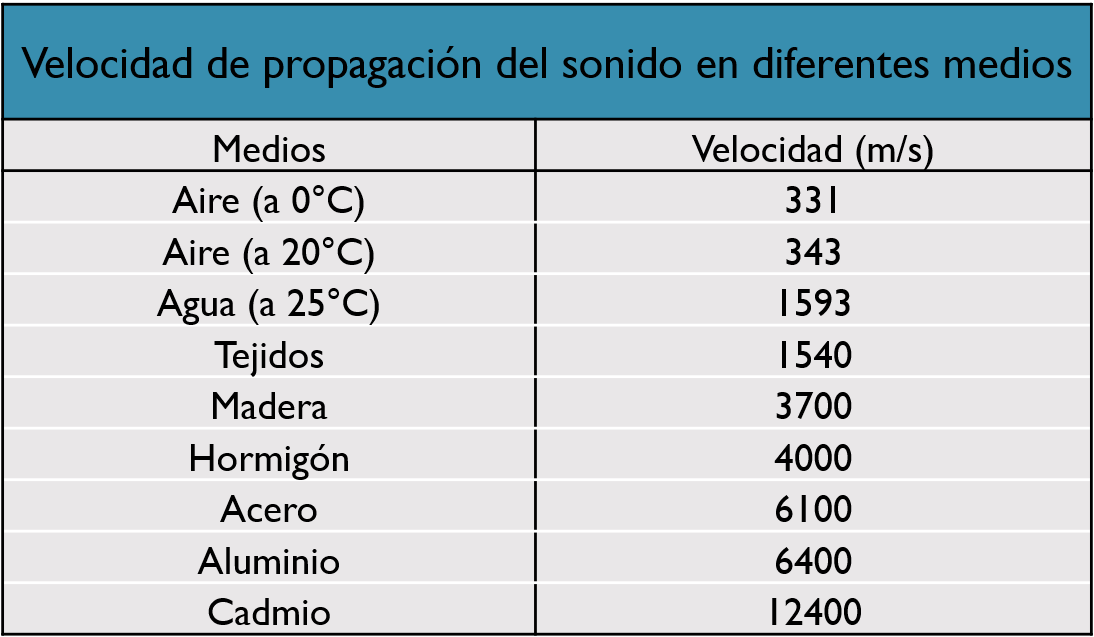
\includegraphics[width=1.0\textwidth]{figures/velocidad_propagacion_sonido.png}
    \caption{Velocidad del sonido en distintos medios de propagación}
    \label{fig:velocidad-propagacion-sonido}
\end{figure}


\subsection{Ejemplo guiado: relación distancia–velocidad–tiempo}
\begin{enumerate}
    \item \textbf{Aplauso a 100 m.} Con $c_{\text{aire}} = 343$ m/s a 20°C:
    \[
    t = \frac{100\,\text{m}}{343\,\text{m/s}} \approx 0.29\,\text{s} \Rightarrow 290\,\text{ms}.
    \]
    Esto explica el retardo entre ver y escuchar fuegos artificiales.
    
    \item \textbf{Sonido en una audiometría de campo libre.} En una cabina de 2 m, el sonido de un audiómetro tarda:
    \[
    t = \frac{2\,\text{m}}{343\,\text{m/s}} \approx 0.006\,\text{s} \Rightarrow 6\,\text{ms}.
    \]
    Este tiempo es imperceptible, pero es clave para calibrar equipos.
\end{enumerate}

\section{Herramientas matemáticas básicas}

\subsection{Funciones}
Una función es como una receta: toma un dato (como el tiempo) y lo transforma en otro (como la presión del sonido). Por ejemplo, la presión del sonido en el tímpano cambia con el tiempo, creando una gráfica que sube y baja, como las ondas del mar.

\subsection{Funciones inversas}
Las funciones inversas ``deshacen'' una operación. En acústica, usamos la inversa del logaritmo para calcular la presión del sonido a partir de un nivel en decibeles (dB).

\subsection{Trigonometría aplicada a ondas}
El sonido se representa con ondas sinusoidales, que son como curvas que suben y bajan regularmente. Por ejemplo, un tono puro (como el pitido de un audiómetro) sigue una forma matemática simple:
\[
x(t) = A \sin(2\pi f t + \varphi).
\]
\begin{itemize}
    \item \textbf{Amplitud ($A$):} Determina el volumen (en pascales, Pa).
    \item \textbf{Frecuencia ($f$):} Indica la altura del sonido (en hertz, Hz). Por ejemplo, 1000 Hz es un tono típico en audiometrías.
    \item \textbf{Periodo ($T$):} Tiempo que tarda la onda en completar un ciclo (en segundos, s). También se calcula como el inverso de la frecuenta ($T = \frac{1}{f}$)
    \item \textbf{Fase ($\varphi$):} Define el punto de partida de la onda (en radianes).
\end{itemize}

\begin{figure}[h]
    \centering
    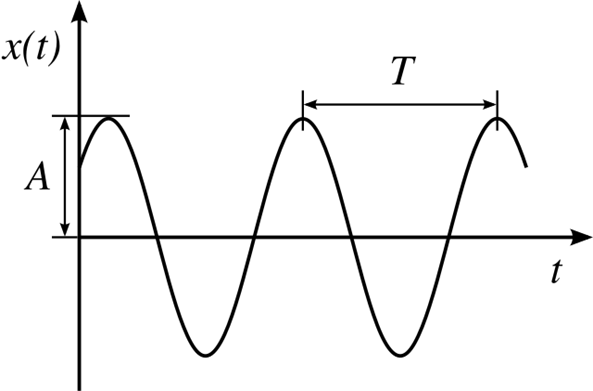
\includegraphics[width=0.8\textwidth]{figures/tono.png}
    \caption{Onda sinusoidal y sus partes.}
    \label{fig:tono-sinusoidal}
\end{figure}

\textbf{Actividad práctica.} Usa una app como Tone Generator (gratis en línea) para escuchar tonos de 250 Hz y 1000 Hz. Nota cómo el de 1000 Hz suena más agudo y prueba cambiar el volumen (amplitud).

\subsection{Logaritmos y decibel}
El oído percibe sonidos desde un susurro (20 $\mu$Pa) hasta un avión (20 Pa), un rango enorme. Los \textbf{decibeles (dB)} usan logaritmos para comprimir este rango:
\[
L_{p}\,[\text{dB}] = 20\,\log_{10}\left(\frac{p}{p_0}\right),\quad p_0 = 20\,\mu\text{Pa}.
\]
Por ejemplo, duplicar la presión del sonido aumenta 6 dB, lo que percibimos como un sonido un poco más fuerte.

\begin{table}[h]
    \centering
    \begin{tabular}{|l|c|}
        \hline
        \textbf{Sonido} & \textbf{Nivel (dB)} \\
        \hline
        Susurro & 20 \\
        Conversación normal & 60 \\
        Tráfico intenso & 80 \\
        Concierto de rock & 100 \\
        Umbral de dolor & 120 \\
        \hline
    \end{tabular}
    \caption{Niveles de decibeles de sonidos cotidianos.}
\end{table}

Video: \href{https://www.youtube.com/watch?v=XLfQpv2ZRPU&ab_channel=MED-EL}{``Understanding Sound Waves | MED-EL''}  

\textbf{Ejemplo.} Si la presión del sonido se duplica (de 20 $\mu$Pa a 40 $\mu$Pa), el nivel aumenta:
\[
\Delta L = 20 \log_{10}(2) \approx 6\,\text{dB}.
\]
Cuando ajustamos el volumen de un audífono para compensar la pérdida auditiva, lo que estamos haciendo es aumentar la presión de salida.

\section{Ejemplos prácticos}

\subsection{Conversión angular}
En acústica, los ángulos (en radianes) describen la fase de una onda. Ejemplo:
\begin{enumerate}[label=\alph*)]
    \item $90^{\circ} = \dfrac{\pi}{2}\,\text{rad}$. Esto representa un cuarto de ciclo en una onda sonora, como el desfase entre dos tonos en una prueba binaural.
    \item $640^{\circ} = 640^{\circ} - 360^{\circ} = 280^{\circ} = \dfrac{14\pi}{9}\,\text{rad}$.
\end{enumerate}

\subsection{Tiempo de viaje del sonido}
\begin{enumerate}
    \item \textbf{Delfín bajo el agua.} Un delfín a 1.5 km emite un click ($c_{\text{agua}} \approx 1500$ m/s):
    \[
    t = \frac{1500\,\text{m}}{1500\,\text{m/s}} = 1\,\text{s}.
    \]
    
    \item \textbf{Localización del sonido.} Si un sonido llega al oído derecho 0.6 ms antes que al izquierdo (distancia entre oídos $\approx 0.2$ m), el tiempo de diferencia es:
    \[
    t = \frac{0.2\,\text{m}}{343\,\text{m/s}} \approx 0.0006\,\text{s} = 0.6\,\text{ms}.
    \]
    Esto ayuda al cerebro a localizar la fuente por la diferencia interaural de tiempo, concepto que veremos en futuras unidades.
\end{enumerate}

\subsection{Nivel de presión sonora}
Para calcular el nivel de presión sonora de un tono de audiometría con presión de 0.02 Pa (20 mPa), debemos usar la siguiente formula:
\[
L_p = 20 \log_{10}\left(\frac{0.02}{20 \times 10^{-6}}\right) = 20 \log_{10}(1000) = 60\,\text{dB}.
\]
Esto corresponde a una conversación normal.

\section{Ejercicios de autoevaluación}
\begin{enumerate}
    \item Indica las unidades SI de densidad (kg/m$^3$), presión (Pa) y frecuencia angular (rad/s).
    \item Mira una gráfica de una onda sonora en una app como Audacity (puedes grabar tu voz). Identifica la amplitud (altura de la onda) y el período (distancia entre picos). Explica cómo se relacionan con el volumen y la altura del sonido.
    \item ¿Cuántos dB aumentan si la presión del sonido se multiplica por 10? (Solución: 20 dB)
    \item Escucha un tono de 500 Hz y otro de 1000 Hz usando una app como Tone Generator. ¿Cuál suena más agudo y por qué?
\end{enumerate}

\section{Glosario}
\begin{description}
    \item[\textbf{Amplitud:}] Máximo cambio de una onda respecto a su valor medio. Determina el volumen del sonido.
    \item[\textbf{Decibel:}] Unidad que mide la intensidad del sonido, basada en logaritmos.
    \item[\textbf{Fase:}] Punto de partida de una onda sonora, que afecta cómo se combina con otras ondas.
    \item[\textbf{Hz:}] Hertz, unidad de frecuencia; un ciclo por segundo.
    \item[\textbf{Onda sonora:}] Vibración que viaja por un medio, como el aire, y lleva el sonido.
    \item[\textbf{Pa:}] Pascal, unidad de presión. Mide la fuerza del sonido en el tímpano.
\end{description}

\section{Resumen}
\begin{itemize}
    \item \textbf{¿Qué es la acústica?} Estudia cómo se generan, propagan y perciben las ondas sonoras, clave en fonoaudiología para audiometrías, audífonos y análisis de voz.
    \item \textbf{Unidades clave:} Longitud (m), tiempo (s), presión (Pa), frecuencia (Hz).
    \item \textbf{Ondas sonoras:} Son longitudinales en el aire (compresiones y rarefacciones) y transversales en sólidos (como el cráneo).
    \item \textbf{Decibeles:} Miden la intensidad del sonido en una escala logarítmica, imitando cómo percibimos los cambios de volumen.
\end{itemize}

\bigskip
\noindent\emph{Conclusión.} Comprender la naturaleza del sonido, las unidades de medida y las herramientas matemáticas básicas es el primer paso para dominar la acústica. Estos conceptos te ayudarán a entender cómo se realizan audiometrías o cómo se analiza la voz de un paciente. En la próxima unidad, exploraremos cómo las leyes de Newton explican el movimiento del tímpano y los huesecillos del oído, conectando la física con la audición.


%%%%%%%%%%%%%%%%%%%%%%%%%%%%%%%%%%%%%%%%%%%%%%%%%%%%%%%%%%%%%%%%%%%%%%%%%%%%%%%%%%%%%%%%%%%%%%%%%%
